%!TEX root = ../dissertation.tex

\chapter{Evaluation}
\label{chapter:evaluation}


In order to evaluate our system, we want to look at its core focus, its
eventual delivery guarantees and overall performance. We not only test our
system by itself, but we also compare it with the current solution tied to
libp2p, entitled Floodsub (currently the default pub-sub implementation within
IPFS). To do this, we rely on the tools previously described in Section
\ref{sec:testbed}.

We start our evaluation by looking into how our testbed is configured in
Section \ref{testbed-configuration}. In Section \ref{dataset}, we document the
dataset we used as well as the transformations necessary to make this data
viable. We then move on to an analysis of the metrics we intended to gather in
Section \ref{metrics}. We are now ready to look into our executions in Section
\ref{executions} as well as its results in Section \ref{results}, where we not
only compare Pulsarcast's performance but also address its new functionalities,
such as the ability to rebuild our topic stream.

\section{Testbed configuration}\label{testbed-configuration}

We designed our test runs to be executed in managed infrastructure (commonly
known as cloud services). For the initial runs and general fine-tuning of the
platform, we relied on Google Cloud's managed Kubernetes solution. Later on,
and for our actual test executions, we ran all of our tests in Microsoft's
Azure Kubernetes solution, thanks to Microsoft and the Azure team, who were kind
enough to support our efforts and offer us free credits.

Our whole setup consisted of a total of 5 VMs acting as Kubernetes Worker
nodes, each with two \acrshort{vcpu}s, 16 \acrshort{gib} of \acrshort{ram} and
32 \acrshort{gib} of storage. In our cluster, besides other operational bits,
we ran 3 Elasticsearch instances, 1 Logstash instance, 1 Kibana and a total of
100 \acrshort{ipfs} Testbed deployments (as described in Section
\ref{subsec:testbed-architecture}). Because we wanted to avoid resource
starvation and to better take advantage of the Kubernetes scheduler, our
testbed deployments allocate 440 \acrshort{mib} of memory per deployment, each
burstable to a maximum of 500 \acrshort{mib}. During our whole test execution,
periodic \acrshort{http} health checks (part of the Kubernetes platform) make
sure our deployments are working accordingly.

Test executions are managed through a single machine, from where all the
commands are sent. During execution, a max of 5 commands are performed in
parallel, with a slight 10-millisecond delay added between each bulk execution.
All the requests are subject to retries. In case of failure, a maximum of 5
attempts can be executed. After these, the failure is registered, and the
execution moves on.

\section{Dataset}\label{dataset}

To test our system accordingly, we wanted a dataset that could simulate a
real-life scenario as much as possible. We chose to use a dataset of
Reddit's~\footnote{\url{https://www.reddit.com/}} comments from
2007~\footnote{\url{http://academictorrents.com/details/7690f71ea949b868080401c749e878f98de34d3d}}~\footnote{\url{https://www.reddit.com/r/datasets/comments/3bxlg7/i_have_every_publicly_available_reddit_comment/}}
consisting of a sample of approximately 25000 comments in a total of 23 topics
(known as subreddits in the platform). For our test runs, the comments
represent events and the topics subreddits.

\subsection{Filtering and Normalisation}\label{subsec:filtering}

Our dataset consisted of line separated JSON structures, each describing a
comment. Given the broad set of data, we started by sampling a set of 25000
messages.  Following this, we needed to first, remove comments from unknown
users (users that had deleted the account at the time when the comments were
scrapped). Next, we had to normalise our user number (reduce the number of
publishers in the dataset to the number of active nodes in our Pulsarcast
system). A final step of data correlation had to take place as well. We ended
up creating a \acrshort{cli} tool that consumed data from this dataset and
generated a document of multiple JSON objects separated by
newlines~\footnote{\url{https://github.com/JGAntunes/pulsarcast-test-harness}},
ready to be used by our ipfs-testbed-cli, described in Section
\ref{subsec:testbed-usage}. Examples of the output produced can be seen in
Section \ref{dataset-output}


\begin{lstlisting}[language=JSON, float, caption={Data example to be used in testbed},label={dataset-output}]
// Topic
{
  "type": "topic",
  "node": "node-71",
  "name": "reddit.com",
  "author": "test-user",
  "totalNumberEvents": 1
}

// User
{
  "type": "user",
  "name": "foobar",
  "node": "node-71",
  "events": [
    {
      "internalId": 0,
      "topic": "reddit.com",
      "body": "test",
      "ups": 1,
      "downs": 0,
      "controversiality": 0
    },
    {
      "internalId": 176,
      "topic": "reddit.com",
      "body": "test-123",
      "ups": 1,
      "downs": 4,
      "controversiality": 0
    }
  ],
  "subscriptions": {
  	"reddit.com": true,
  	"politics": true,
  	"business": true,
	}
}
\end{lstlisting}

\subsection{Data distribution}\label{subsec:data-distribution}

The following graphs give us a distribution analysis of events published per
topic (Figure \ref{fig:events-to-be-publisher-per-topic}), subscriptions per
topic (Figure \ref{fig:subscriptions-per-topic}) and subscription distribution
per nodes (Figure \ref{fig:subscription-distribution-per-node}). Given our
dataset choice, we aimed for a non-uniform subscription distribution per topic
and, as it would be expected in a real-world scenario, the distribution of
events follows a power law based on their popularity. 

\begin{figure}[!htb]
  \centering
  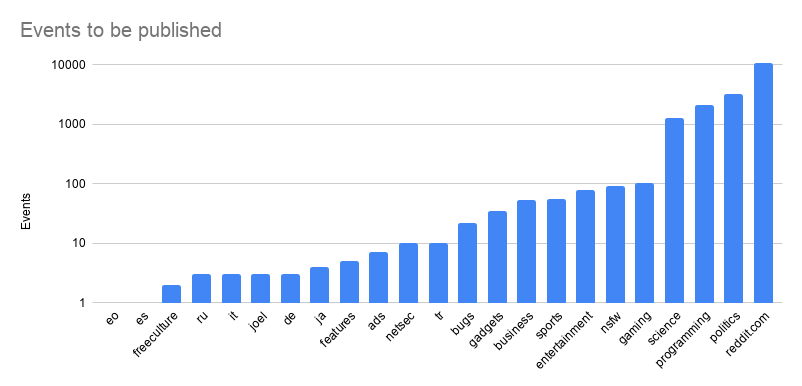
\includegraphics[width=0.8\textwidth]{img/events-to-be-publisher-per-topic.png}
  \caption{Event distribution per topic with log scale}
  \label{fig:events-to-be-publisher-per-topic}
\end{figure}

\begin{figure}[!htb]
  \centering
  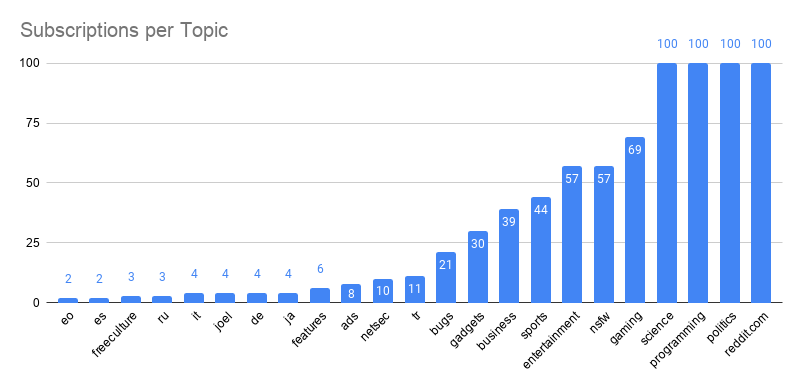
\includegraphics[width=0.8\textwidth]{img/subscriptions-per-topic.png}
  \caption{Subscription distribution per topic}
  \label{fig:subscriptions-per-topic}
\end{figure}

\begin{figure}[!htb]
  \centering
  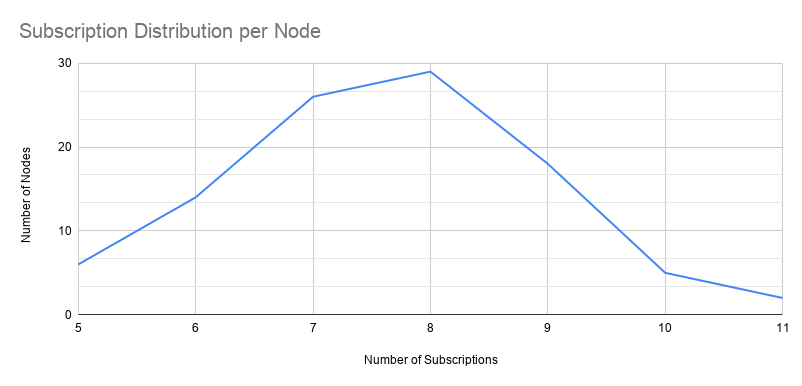
\includegraphics[width=0.8\textwidth]{img/subscription-distribution-per-node.png}
  \caption{Subscription distribution per number of nodes}
  \label{fig:subscription-distribution-per-node}
\end{figure}

\section{Metrics}\label{metrics}

For each execution, we look to extract two key groups of data: resource usage
data and \acrshort{qos} data. The following list describes these in more detail:

\begin{itemize}
  \item Resource usage as a total in the whole cluster, and per-node (95/99
  percentile and average)
  \begin{itemize}
    \item \acrshort{cpu} Usage (\acrshort{cpu} number)
    \item Memory Usage (\acrshort{gib})
    \item Network Usage (\acrshort{mib} transmitted)
  \end{itemize}
  \item \acrshort{qos}
  \begin{itemize}
    \item Events published by topic and in total
    \item Events received by topic and in total
    \item Percentage of subscriptions fulfilled based on the number of events
    successfully published
    \item Percentage of subscriptions fulfilled based on the total number of events
    injected in the system
    \item Number of \acrshort{rpc} messages sent per topic and in total
    \item Average, standard deviation and percentiles (99/95) of the number of \acrshort{rpc} messages received and sent by each node
  \end{itemize}
\end{itemize}

We measure the subscription coverage (number of subscriptions fulfilled)
through two distinct metrics. The percentage of fulfillment having the number
of events effectively published as a reference and the percentage of
fulfillment having the total number of events injected into the system as
reference. Given Pulsarcast's nature, when an event is injected into the
system, depending on the topic configuration, it may need to be propagated
through the dissemination trees before being effectively published
(\emph{request to publish}). It also needs to be persisted in the
\acrshort{dht}. Having two different metrics allows us to better analyse and
distinguish the different behaviours of the system.

It is essential to keep in mind that some of the metrics under the \acrshort{qos} group
only make sense in Pulsarcast test runs, hence will be ignored when running the
baseline Floodsub solution.

\section{Executions}\label{executions}

We have devised a total of 6 test executions we wanted to go through and
compare results. Starting with the three base scenarios, we wanted to test:

\begin{itemize}
  \item Pulsarcast without order delivery guarantee
  \item Pulsarcast with order delivery guarantee
  \item Floodsub (baseline solution)
\end{itemize}

For the first one, we run a scenario where every created topic in Pulsarcast
allows every participating node to publish events. For the second execution, we
configure the topics so that only the creator of the topic is allowed to
publish, all the events from other nodes will need to be forwarded as a request
to publish (as described in Section
\ref{subsec:publishing-and-event-dissemination}).  Floodsub was used as it is,
as no configuration is required. 

For each of the executions described above, we performed two tests, one without
any network disturbances, and another using Toxiproxy's features, adding a
latency of 500 milliseconds and 300 milliseconds of jitter to every incoming
\acrshort{tcp} packet. 

\section{Results}\label{results}

In this section we will evaluate the results for each of the executions we
described, followed by a comparison and analysis of these.

\subsection{Pulsarcast With Order Guarantee}\label{subsec:pulsarcast-with-order-guarantee}

For this test, we explored how the Pulsarcast system performed when only a
single node (the creator of the topic), was allowed to effectively publish
events. The execution took a total of 38 minutes. However, at the 10-minute
mark, one of our nodes (the root node for the reddit.com topic) became
unresponsive due to the load it was dealing with and the lack of \acrshort{cpu} power to
handle it, eventually leading the Kubernetes scheduler to restart it.  Given
that Pulsarcast does not provide a recovery mechanism for root nodes of a topic
out of the box and the fact that this was the only node allowed to publish (for
this specific topic), we ended up seeing a clear impact in our results.

\begin{figure}[!htb]
  \centering
  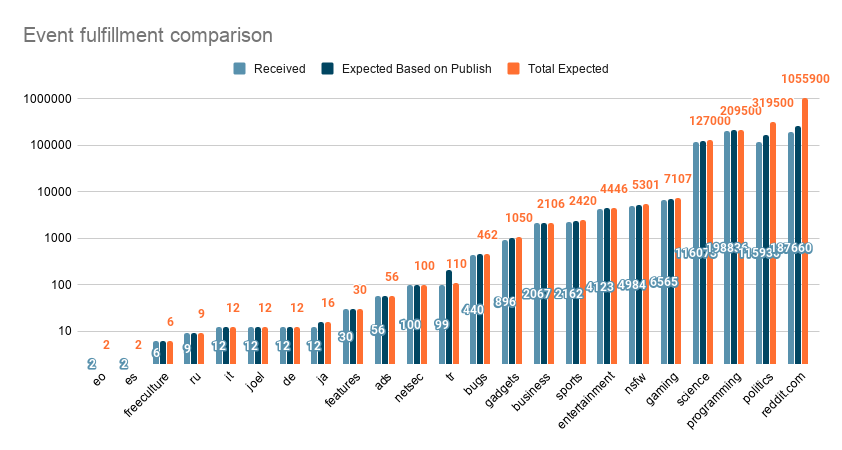
\includegraphics[width=0.8\textwidth]{img/graph-pulsarcast-order-event-fulfillment-comparison.png}
  \caption{Pulsarcast with order guarantee - Comparison of of events fulfilled by topic in a log scale}
  \label{fig:graph-pulsarcast-order-event-fulfillment-comparison}
\end{figure}

\begin{figure}[!htb]
  \centering
  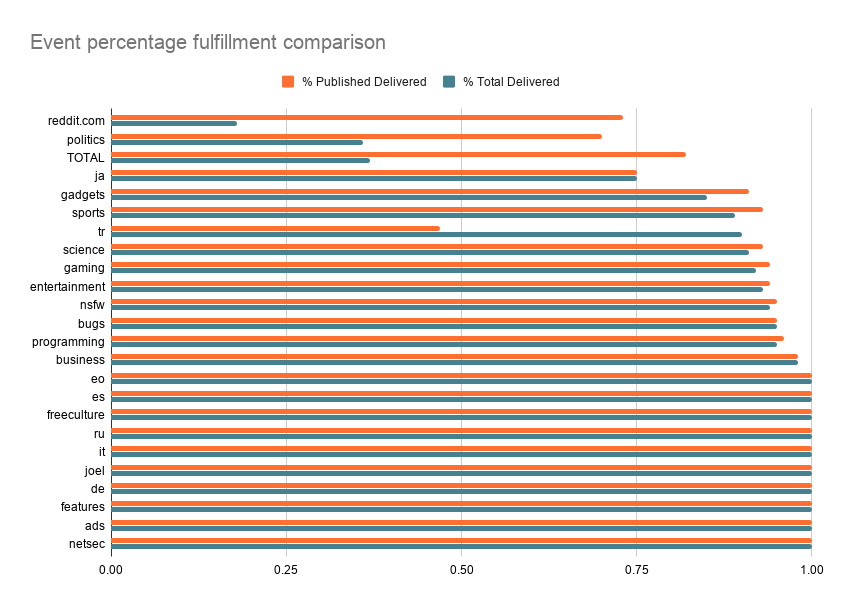
\includegraphics[width=0.8\textwidth]{img/graph-pulsarcast-order-event-percentage-fulfillment-comparison.png}
  \caption{Pulsarcast with order guarantee - Comparison of percentage of events fulfilled by topic}
  \label{fig:graph-pulsarcast-order-event-percentage-fulfillment-comparison}
\end{figure}

Looking at Figures
\ref{fig:graph-pulsarcast-order-event-fulfillment-comparison} and
\ref{fig:graph-pulsarcast-order-event-percentage-fulfillment-comparison} we can
see that, of the total of events injected into the system, Pulsarcast fulfilled
37\% of its subscriptions. Having the number of events effectively published as
reference (the \emph{requests to publish} that reach the topic root node and
single publisher), Pulsarcast fulfilled 80\% of its subscriptions. The
disparity between both values clearly highlights that we suffered from the
early drop-out node. Given that this same node was the root node for the most
popular topic (\emph{reddit.com}), once it became unresponsive and restarted,
all further requests to publish failed. However, it is important to notice
that from the all the events published, our system successfully covered 80\% of
its subscribers, which is a fairly high success rate.

\begin{figure}[!htb]
  \centering
  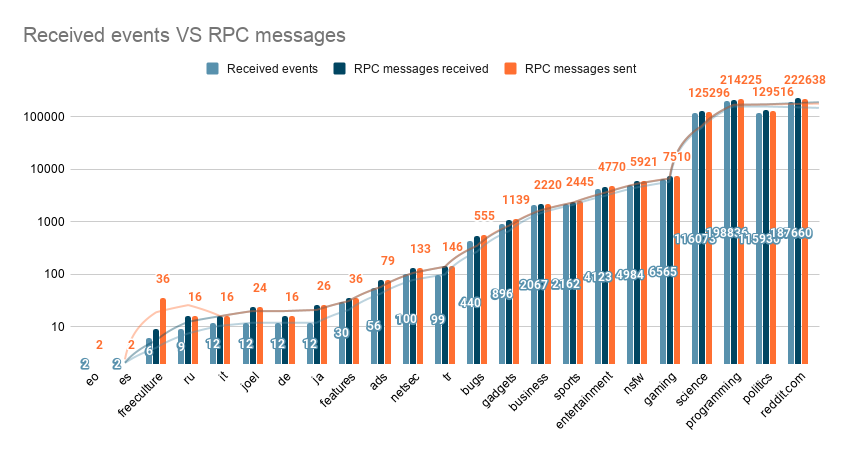
\includegraphics[width=0.8\textwidth]{img/graph-pulsarcast-order-rpc.png}
  \caption{Pulsarcast with order guarantee - Comparison of events received and \acrshort{rpc} injected in the system}
  \label{fig:graph-pulsarcast-order-rpc}
\end{figure}

Considering Figure \ref{fig:graph-pulsarcast-order-rpc}, we see that the
\acrshort{rpc} messages injected in the system grow linearly with the number of
events received.

Table \ref{table:pulsarcast-order} provides an overview of the Memory and
Network utilisation by node. Given these grew linearly through the test
execution, we are only presenting the final values. We also provide an \acrshort{rpc}
message analysis by node. Despite having a low consumption overall (Network and
Memory wise), we can see the presence of a relatively large set of outliers, a
possible consequence of the unfairness of this execution, given its tendency to
overload the owners of the topics. Now, looking at the graph in Figure
\ref{fig:graph-pulsarcast-order-cpu} which shows us the \acrshort{cpu} usage across time,
we can see the same outlier pattern as before, as well as the moment (at the 10
minute mark) when the \acrshort{cpu} usage picked for the node which eventually became
unresponsive.

\begin{table}[!htb]
\caption{Pulsarcast with order guarantee - Resource utilisation metrics per node}
\label{table:pulsarcast-order}
  \begin{center}
   \begin{tabular}{|c| c c c c c|} 
    % \label{tab:pulsarcast-order}
   \hline
   / & P95 & P99 & Average & Standard Deviation & Total \\ [0.5ex] 
   \hline\hline
   Memory (\acrshort{gib}) & 0.207 & 0.358 & 0.178 & [NA] & 17.84 \\
   \hline
   Network (\acrshort{mib}) & 26.26 & 99.41 & 10.5 & [NA] & 1050.4 \\
   \hline
   \acrshort{rpc} Messages Received & 8440 & 8961 & 7315.18 & 1205.68 & [NA] \\
   \hline
   \acrshort{rpc} Messages Sent & 33655.5 & 80058.5 & 5889.29 & 13921.84 & [NA] \\ [1ex] 
   \hline
  \end{tabular}
  \end{center}
\end{table}

\begin{figure}[!htb]
  \centering
  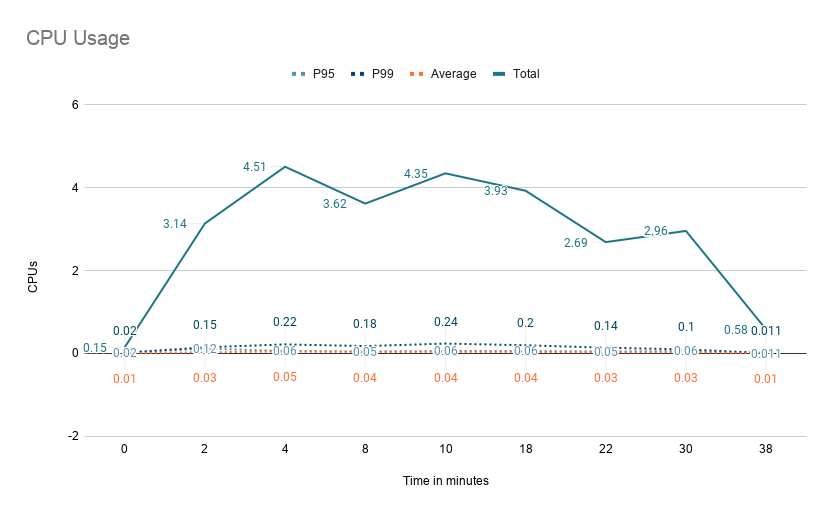
\includegraphics[width=0.8\textwidth]{img/graph-pulsarcast-order-cpu.png}
  \caption{Pulsarcast with order guarantee - \acrshort{cpu} usage across time}
  \label{fig:graph-pulsarcast-order-cpu}
\end{figure}

\subsection{Pulsarcast Without Order Guarantee}\label{subsec:pulsarcast-without-order-guarantee}

We will now be looking at the Pulsarcast scenario without order guarantee,
which entails that now every node is allowed to publish messages to topics it
is subscribed to. For this scenario, the execution took a total of 85 minutes.

\begin{figure}[!htb]
  \centering
  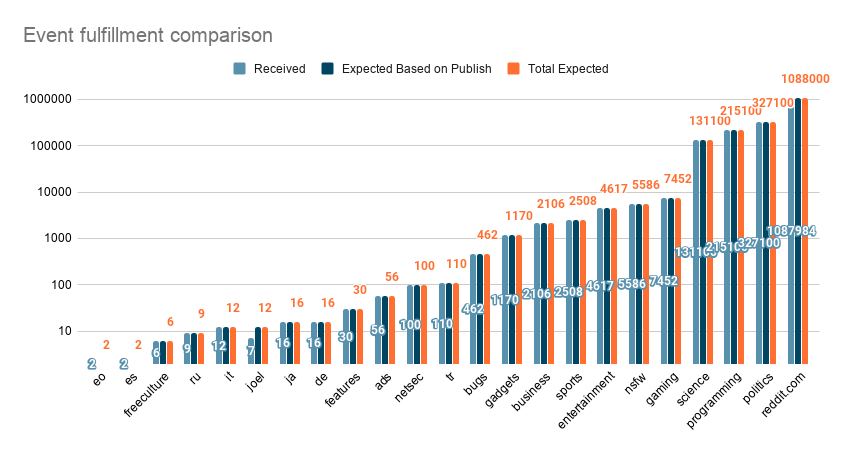
\includegraphics[width=0.8\textwidth]{img/graph-pulsarcast-event-fulfillment-comparison.png}
  \caption{Pulsarcast without order guarantee - Comparison of of events fulfilled by topic in a log scale}
  \label{fig:graph-pulsarcast-event-fulfillment-comparison}
\end{figure}

\begin{figure}[!htb]
  \centering
  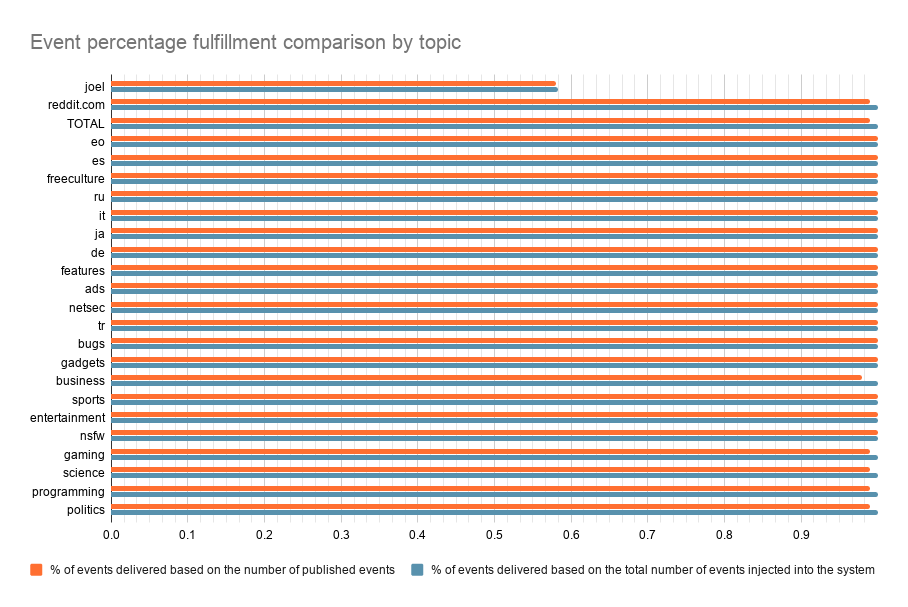
\includegraphics[width=0.8\textwidth]{img/graph-pulsarcast-event-percentage-fulfillment-comparison.png}
  \caption{Pulsarcast without order guarantee - Comparison of percentage of events fulfilled by topic}
  \label{fig:graph-pulsarcast-event-percentage-fulfillment-comparison}
\end{figure}

Looking at Figures \ref{fig:graph-pulsarcast-event-fulfillment-comparison} and
\ref{fig:graph-pulsarcast-event-percentage-fulfillment-comparison} we can see
that, of the total of events injected into the system, Pulsarcast fulfilled
99\% of its subscriptions. Taking the events effectively published as
reference, Pulsarcast fulfilled 99\% of its subscriptions. A clear difference
to the previous execution.

\begin{figure}[!htb]
  \centering
  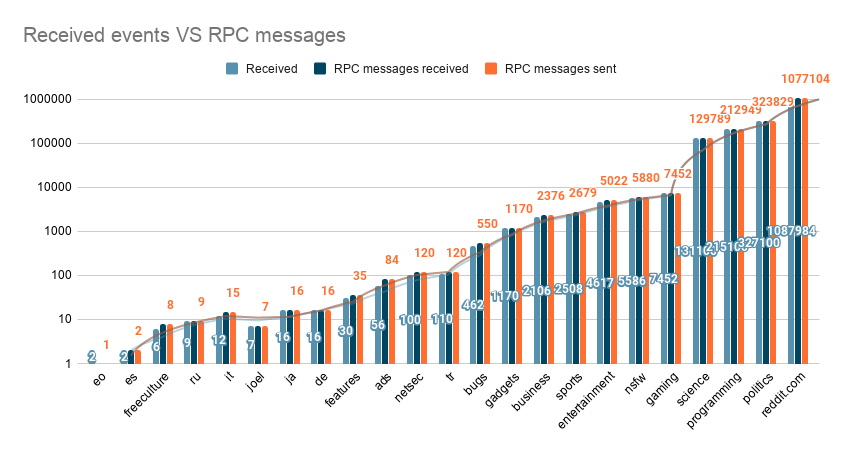
\includegraphics[width=0.8\textwidth]{img/graph-pulsarcast-rpc.png}
  \caption{Pulsarcast without order guarantee - Comparison of events received and \acrshort{rpc} injected in the system}
  \label{fig:graph-pulsarcast-rpc}
\end{figure}

Considering Figure \ref{fig:graph-pulsarcast-rpc}, we see that the \acrshort{rpc} messages
injected in the system grow linearly with the number of events received.

Table \ref{table:pulsarcast} provides an overview of the Memory and Network
utilisation by node. As previously, these grew linearly throw the test
execution we are only presenting the final values. We also provide an
\acrshort{rpc} message analysis by node. Memory wise, we have an evenly
distributed consumption across nodes. In terms of network, we still have a
couple of outliers, which can probably be explained by how the dissemination
trees were formed.  Now, looking at the graph in Figure
\ref{fig:graph-pulsarcast-cpu} which shows us the \acrshort{cpu} usage across
time, we can see a low \acrshort{cpu} usage in total. As for the distribution,
we can see a small set of outliers across time as these were the nodes
publishing events at the time (explainable due to our heavy dependence on
cryptographic hash functions).  Overall though we see a clear difference in how
resource consumption is more evenly distributed compared to the order guarantee
experiment.

\begin{table}[!htb]
\caption{Pulsarcast without order guarantee - Resource utilisation metrics per node}
\label{table:pulsarcast}
  \begin{center}
   \begin{tabular}{|c| c c c c c|} 
    % \label{tab:pulsarcast-order}
   \hline
   / & P95 & P99 & Average & Standard Deviation & Total \\ [0.5ex] 
   \hline\hline
   Memory (\acrshort{gib}) & 0.369 & 0.378 & 0.319 & [NA] & 31.924 \\
   \hline
   Network (\acrshort{mib}) & 49.143 & 129.82 & 22.377 & [NA] & 2237.736 \\
   \hline
   \acrshort{rpc} Messages Received & 17843 & 17889.5 & 17708.4 & 85.92 & [NA] \\
   \hline
   \acrshort{rpc} Messages Sent & 84055 & 267124.5 & 17708.4 & 46329.87 & [NA] \\ [1ex] 
   \hline
  \end{tabular}
  \end{center}
\end{table}

\begin{figure}[!htb]
  \centering
  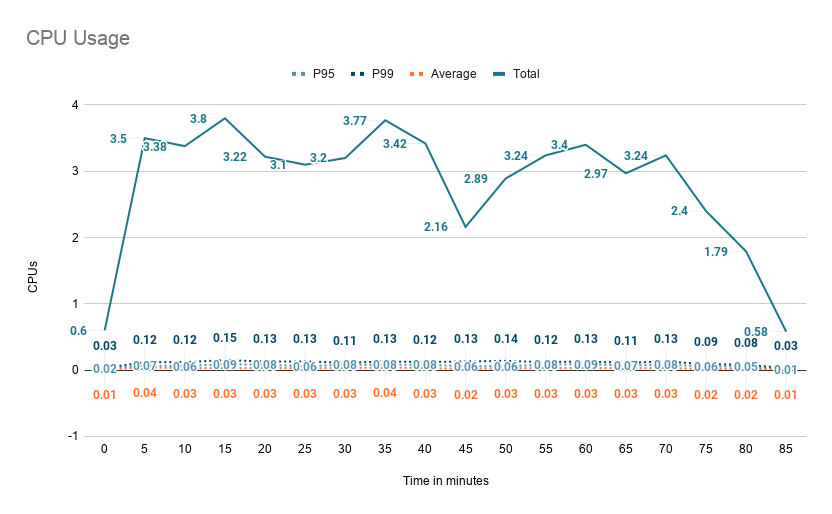
\includegraphics[width=0.8\textwidth]{img/graph-pulsarcast-cpu.png}
  \caption{Pulsarcast without order guarantee - \acrshort{cpu} usage across time}
  \label{fig:graph-pulsarcast-cpu}
\end{figure}

\subsection{Floodsub}\label{subsec:floodsub}

Our next execution is a test run using Floodsub. The main goal of it is to act
as a baseline for our system. It took a total of 70 minutes to finish. However,
the whole network was unable to cope with the load of our execution and 10
minutes after our test started nodes became unresponsive and either crashed or
were repeatedly terminated by our Kubernetes scheduler, eventually hitting a
minimum of 15 nodes running. It took 50 minutes for the network to fully
recover and have 100 nodes running again, only for the execution to finish 10
minutes later. This is a clear indicator of the Floodsub inability to handle
the same workload as Pulsarcast did in the previous executions. Which is
expected, as the way Floodsub operates is by forwarding messages to all of its
peers, creating a huge amount of strain in the network (both CPU wise and in
network data transmission).

\begin{figure}[!htb]
  \centering
  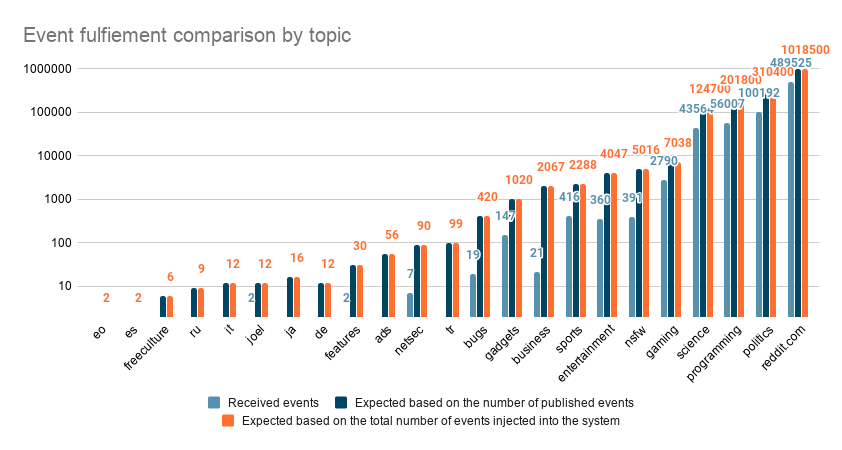
\includegraphics[width=0.8\textwidth]{img/graph-floodsub-event-fulfillment-comparison.png}
  \caption{Floodsub - Comparison of of events fulfilled by topic in a log scale}
  \label{fig:graph-floodsub-event-fulfillment-comparison}
\end{figure}

\begin{figure}[!htb]
  \centering
  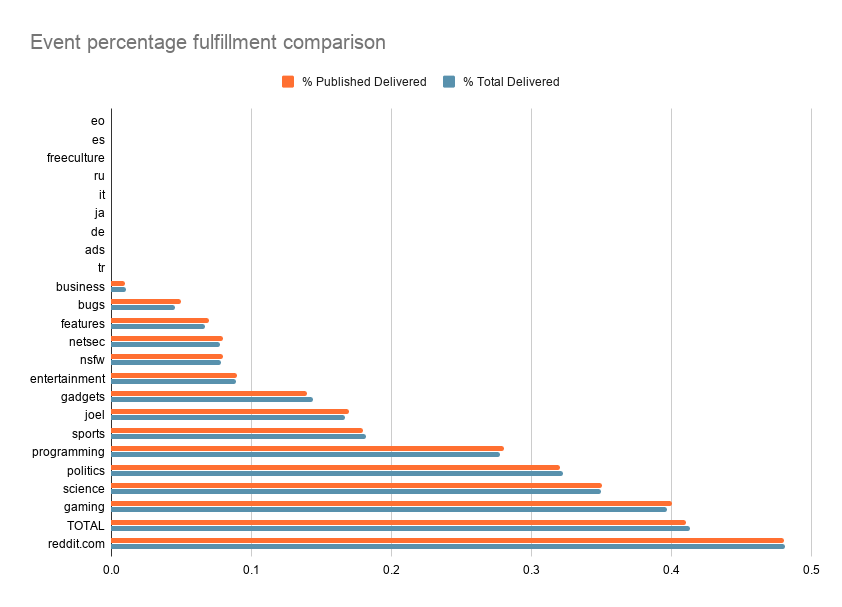
\includegraphics[width=0.8\textwidth]{img/graph-floodsub-event-percentage-fulfillment-comparison.png}
  \caption{Floodsub - Comparison of percentage of events fulfilled by topic}
  \label{fig:graph-floodsub-event-percentage-fulfillment-comparison}
\end{figure}

Looking at Figures \ref{fig:graph-floodsub-event-fulfillment-comparison} and
\ref{fig:graph-floodsub-event-percentage-fulfillment-comparison} we can see
that, of the total of events injected into the system, Floodsub fulfilled 41\%
of its subscriptions. The same goes if we consider the events successfully
published as the base reference. Analysing these values, we can see we have a
slightly higher fulfilment percentage when comparing with Pulsarcast with order
guarantee. However, a way lower fulfilment percentage comparing with the
execution of Pulsarcast without order guarantee (which is the QoS level offered
by Floodsub). Another thing to take into account is the way Floodsub performed
on a per topic basis, failing to fulfil a  whole range of low popularity
topics.

Table \ref{table:floodsub} provides an overview of the Network utilisation by
node. It grew linearly throw the test execution, and as such, we are only
presenting the final values. Memory wise, contrary to previous executions, it
fluctuated during the test (caused by the node failures) as such we are
presenting these values in the form of a graph in Figure
\ref{fig:graph-floodsub-memory}. The \acrshort{cpu} usage can be seen in Figure
\ref{fig:graph-floodsub-cpu}. Starting by analysing the network usage, we see a
total value of 6552 \acrshort{mib} transmitted, averaging at 66 \acrshort{mib}
per node. This result comes as no surprise, given Floodsub's algorithm, which
repeatedly retransmits the same event to all the peers each node is connected
to. Now, looking at both the memory and \acrshort{cpu} evolution across time,
these suffered from the node crashes.  However, looking at the \acrshort{cpu}
usage, we see a total resource consumption greater than previous executions, as
well as a more uniform distribution across nodes than, for example, the
Pulsarcast order guarantee execution. With a P99 sometimes greater than 0.2,
this explains the node failures across the test.

\begin{table}[!htb]
\caption{Floodsub - Resource utilisation metrics per node}
\label{table:floodsub}
  \begin{center}
   \begin{tabular}{|c| c c c c|} 
    % \label{tab:pulsarcast-order}
   \hline
   / & P95 & P99 & Average & Total \\ [0.5ex] 
   \hline\hline
   Network (\acrshort{mib}) & 105.29 & 133.9 & 65.52 & 6552.4 \\
   \hline
  \end{tabular}
  \end{center}
\end{table}

\begin{figure}[!htb]
  \centering
  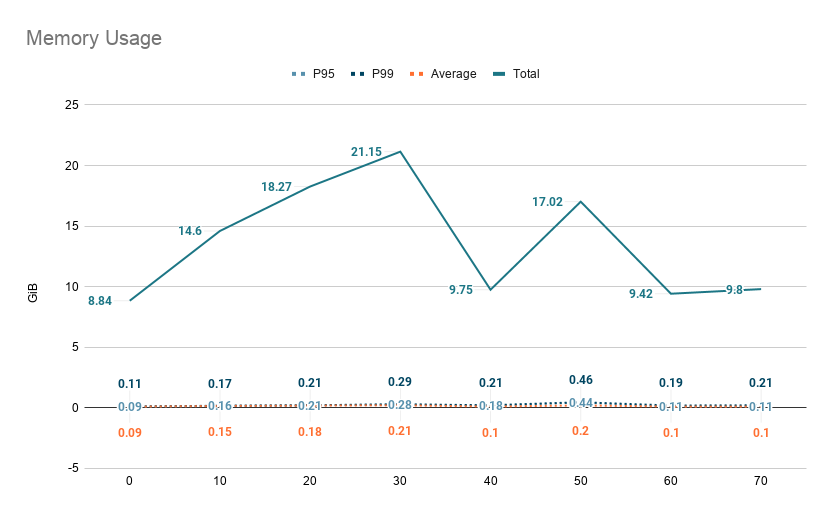
\includegraphics[width=0.8\textwidth]{img/graph-floodsub-memory.png}
  \caption{Floodsub - Memory usage across time}
  \label{fig:graph-floodsub-memory}
\end{figure}

\begin{figure}[!htb]
  \centering
  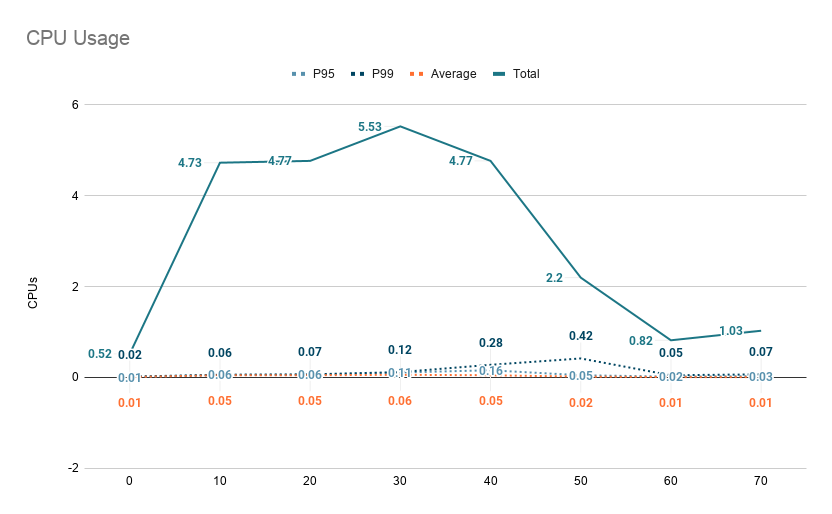
\includegraphics[width=0.8\textwidth]{img/graph-floodsub-cpu.png}
  \caption{Floodsub - \acrshort{cpu} usage across time}
  \label{fig:graph-floodsub-cpu}
\end{figure}

\subsection{Pulsarcast With Order Guarantee and Latency}\label{subsec:pulsarcast-with-order-guarantee-and-latency}

For our next test, we explored how the Pulsarcast system performed when only a
single node (the creator of the topic), was allowed to effectively publish
events but, with a caveat, all the nodes were injected with an inbound latency
of 500 ms and 300 ms of jitter. The execution took a total of 226 minutes,
however, similar to what happened in the latency-free experiment, two of our
nodes (the root nodes for the reddit.com and politics topics) became
unresponsive at the 48 minutes and 196-minute marks respectively. This result
was due to the load both nodes were dealing with and the lack of \acrshort{cpu} power to
handle it, eventually leading the Kubernetes scheduler to restart them. These
two events ended up interfering with our results, just as it happened in the
latency-free experiment.

\begin{figure}[!htb]
  \centering
  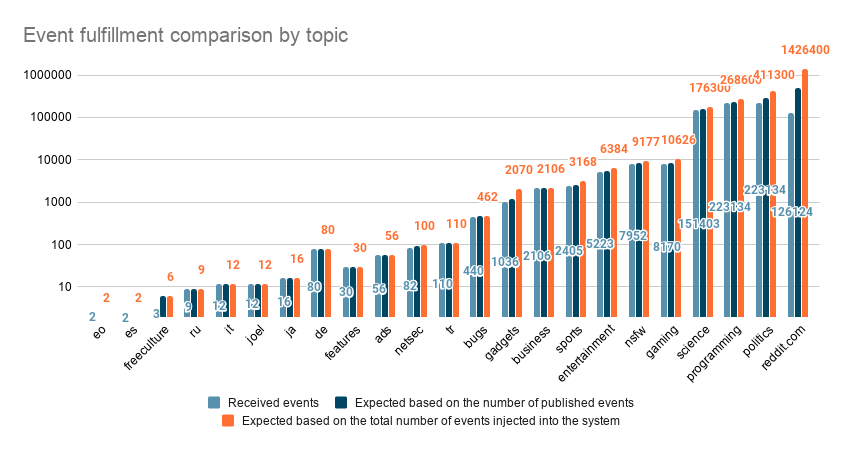
\includegraphics[width=0.8\textwidth]{img/graph-pulsarcast-order-latency-event-fulfillment-comparison.png}
  \caption{Pulsarcast with order guarantee and latency - Comparison of of events fulfilled by topic in a log scale}
  \label{fig:graph-pulsarcast-order-latency-event-fulfillment-comparison}
\end{figure}

\begin{figure}[!htb]
  \centering
  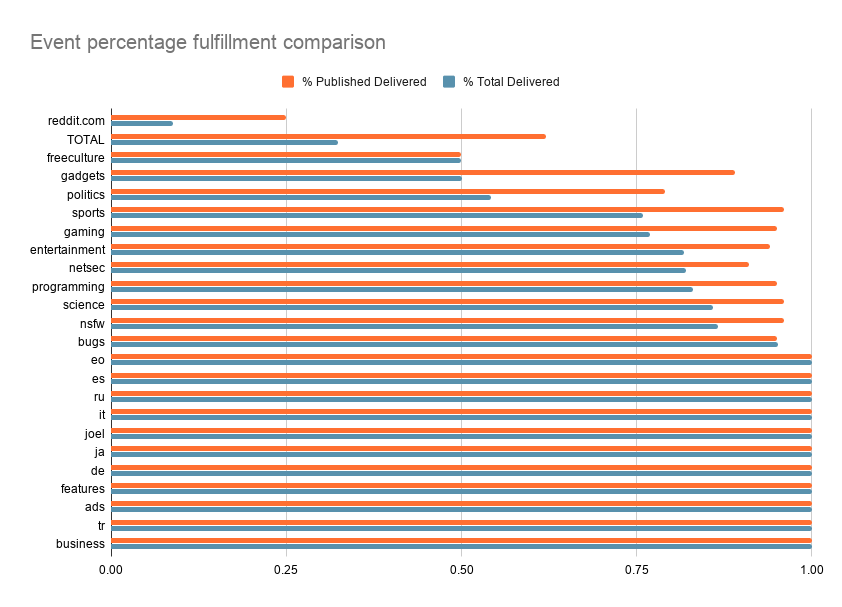
\includegraphics[width=0.8\textwidth]{img/graph-pulsarcast-order-latency-event-percentage-fulfillment-comparison.png}
  \caption{Pulsarcast with order guarantee and latency - Comparison of percentage of events fulfilled by topic}
  \label{fig:graph-pulsarcast-order-latency-event-percentage-fulfillment-comparison}
\end{figure}

Analysing Figures
\ref{fig:graph-pulsarcast-order-latency-event-fulfillment-comparison} and
\ref{fig:graph-pulsarcast-order-latency-event-percentage-fulfillment-comparison}
we can see that, of the total of events injected into the system, Pulsarcast
fulfilled 32\% of its subscriptions. Having the events effectively published
into the system as a reference, Pulsarcast fulfilled 62\% of its subscriptions.
Similar to what was described in Section
\ref{subsec:pulsarcast-with-order-guarantee}, the nodes that restarted are the
key reason for these lower percentages, given both were the root nodes for our
most popular topics \emph{reddit.com} and \emph{politics}. All the requests to
publish sent after the restart ended up rendering no effect. One interesting
fact from this experiment is that, even though we increased the latency of the
underlying network, the \acrshort{qos} did not suffer a clear impact.  However,
the whole experiment took a long time to fulfil. This is because the Pulsarcast
implementation, when running the commands we discussed, waits on the initial
propagation of events/topics before returning control to the caller (and
consequently replying to the clients of our \acrshort{http} \acrshort{api}).
This ended up working as a backpressure system for our test suite.

\begin{figure}[!htb]
  \centering
  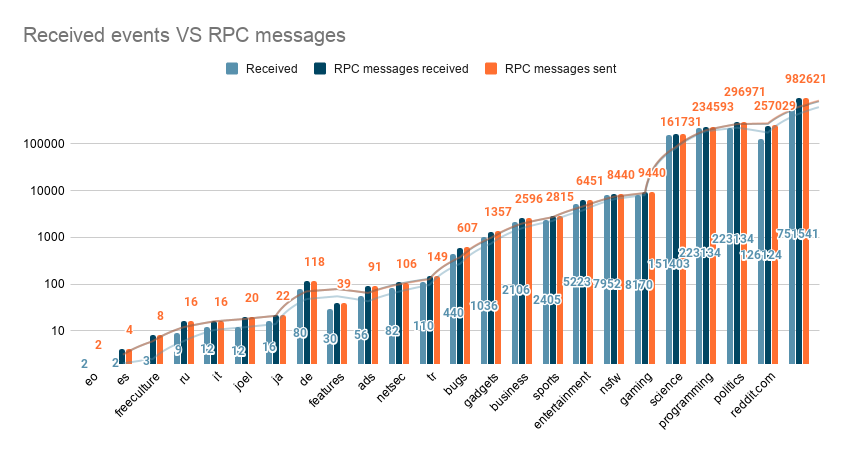
\includegraphics[width=0.8\textwidth]{img/graph-pulsarcast-order-latency-rpc.png}
  \caption{Pulsarcast with order guarantee and latency - Comparison of events received and \acrshort{rpc} injected in the system}
  \label{fig:graph-pulsarcast-order-latency-rpc}
\end{figure}


As expected, Figure \ref{fig:graph-pulsarcast-order-latency-rpc} shows us that
the \acrshort{rpc} messages injected in the system grow linearly with the number of events
received.

Table \ref{table:pulsarcast-order-latency} provides an overview of the Memory
and Network utilisation by node. Similar to the previous experiments, these
grew linearly throughout the test execution. As such, we are only presenting
the final values. We also provide an \acrshort{rpc} message analysis by node. Just as it
happened in the latency-free execution, we have an overall low resource
consumption, however, the presence of a clear set of outliers shows how unfair
the network can be when order guarantee is enforced.

The graph in Figure \ref{fig:graph-pulsarcast-order-latency-cpu} shows us the
\acrshort{cpu} consumption per node during the first 60 minutes. For simplicity
sake, we only show a slice of the execution given that that same pattern
repeats until the end of the test run. In it, we can see a spike pattern,
consequence of the network latency induced. Each spike represented when the
overall network was busy handling events. It is during one of these spikes that
our first node became unresponsive (at the 48-minute mark) as well as the
second node later on.

\begin{table}[!htb]
\caption{Pulsarcast with order guarantee and latency - Resource utilisation metrics per node}
\label{table:pulsarcast-order-latency}
  \begin{center}
   \begin{tabular}{|c| c c c c c|} 
    % \label{tab:pulsarcast-order}
   \hline
   / & P95 & P99 & Average & Standard Deviation & Total \\ [0.5ex] 
   \hline\hline
   Memory (\acrshort{gib}) & 0.23 & 0.35 & 0.2 & [NA] & 19.99 \\
   \hline
   Network (\acrshort{mib}) & 37.05 & 150.18 & 15.96 & [NA] & 1595.6 \\
   \hline
   \acrshort{rpc} Messages Received & 11731 & 11862.5 & 9647.13 & 1767.25 & [NA] \\
   \hline
   \acrshort{rpc} Messages Sent & 43018.5 & 106661.5 & 8215.28 & 18268.99 & [NA] \\ [1ex] 
   \hline
  \end{tabular}
  \end{center}
\end{table}

\begin{figure}[!htb]
  \centering
  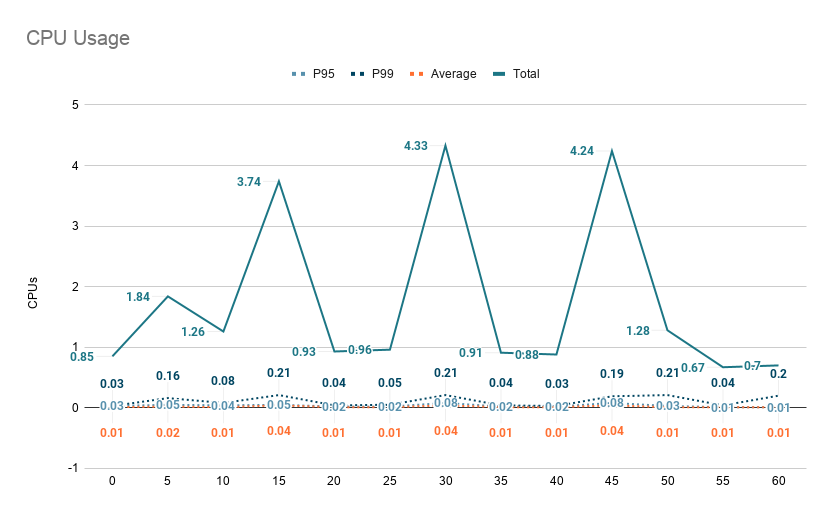
\includegraphics[width=0.8\textwidth]{img/graph-pulsarcast-order-latency-cpu.png}
  \caption{Pulsarcast with order guarantee and latency - \acrshort{cpu} usage across time}
  \label{fig:graph-pulsarcast-order-latency-cpu}
\end{figure}

\subsection{Pulsarcast Without Order Guarantee and Latency}\label{subsec:pulsarcast-without-order-guarantee-and-latency}

The next execution explores how the Pulsarcast system performed when all the
nodes were allowed to publish but, just as in the previous experiment, all the
nodes experienced an inbound network latency of 500 ms and 300 ms of jitter.
The execution took a total of 13 hours, our most lengthened experiment from all
of the scenarios. Just as we described before, commands in Pulsarcast wait for
the initial events/topics to be injected in the network before returning
control to the client. For topics where everyone is allowed to publish (this
execution exactly), this will mean that for each event published, Pulsarcast
will also wait for the event to be persisted in the \acrshort{dht}. Similar to
what happened in Section
\ref{subsec:pulsarcast-with-order-guarantee-and-latency}, this behaviour
created a natural backpressure mechanism. Unfortunately for us, we are running
on a tight set of specifications, and currently all the state is kept in
memory. This meant that, when the execution ended up running longer than what
we originally predicted, two nodes were terminated by our Kubernetes scheduler
due to shortage of memory resources at the 9-hour mark.

\begin{figure}[!htb]
  \centering
  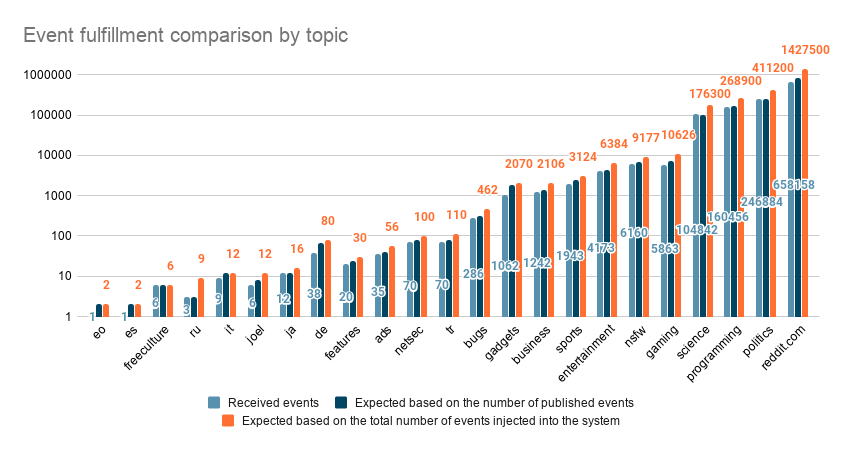
\includegraphics[width=0.8\textwidth]{img/graph-pulsarcast-latency-event-fulfillment-comparison.png}
  \caption{Pulsarcast without order guarantee and latency - Comparison of of events fulfilled by topic in a log scale}
  \label{fig:graph-pulsarcast-latency-event-fulfillment-comparison}
\end{figure}

\begin{figure}[!htb]
  \centering
  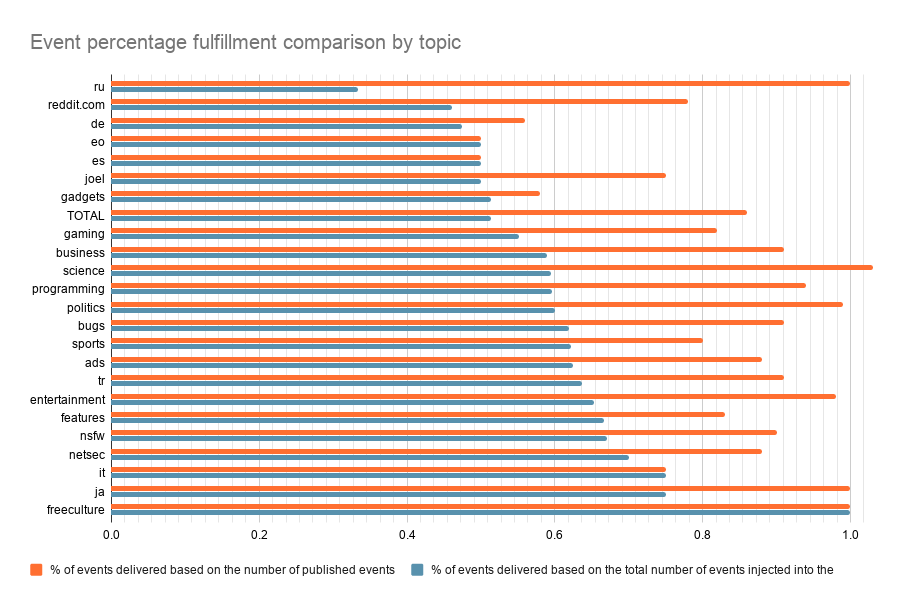
\includegraphics[width=0.8\textwidth]{img/graph-pulsarcast-latency-event-percentage-fulfillment-comparison.png}
  \caption{Pulsarcast without order guarantee and latency - Comparison of percentage of events fulfilled by topic}
  \label{fig:graph-pulsarcast-latency-event-percentage-fulfillment-comparison}
\end{figure}

Looking at Figures
\ref{fig:graph-pulsarcast-latency-event-fulfillment-comparison} and
\ref{fig:graph-pulsarcast-latency-event-percentage-fulfillment-comparison} we
can see that, of the total of events injected into the system, Pulsarcast
fulfilled 51\% of its subscriptions. Having the events effectively published
into the system as a reference, Pulsarcast fulfilled 86\% of its subscriptions.
Although somewhat low for the total of events expected to be published, our
fulfilment rate for events actually published was quite high (86\%). The
discrepancy between these two values can, of course, be explained.  The two
nodes that restarted have had some impact in the results obtained but that is
not the only explanation, as in this scenario every node is capable of
publishing events. As it has been previously covered, Pulsarcast has a natural
backpressuring system consequence of the way we wait for an initial response
when disseminating events/topics or persisting state in the \acrshort{dht}.
With the system running on top of a debilitated network, this meant that not
even the retries in our test suite could cover for network timeouts and
failures.  This negatively impacted some events, given we were effectively
unable to publish them as the nodes failed to meet the necessary pre-requisites
(persist it in the \acrshort{dht} and disseminate it).

\begin{figure}[!htb]
  \centering
  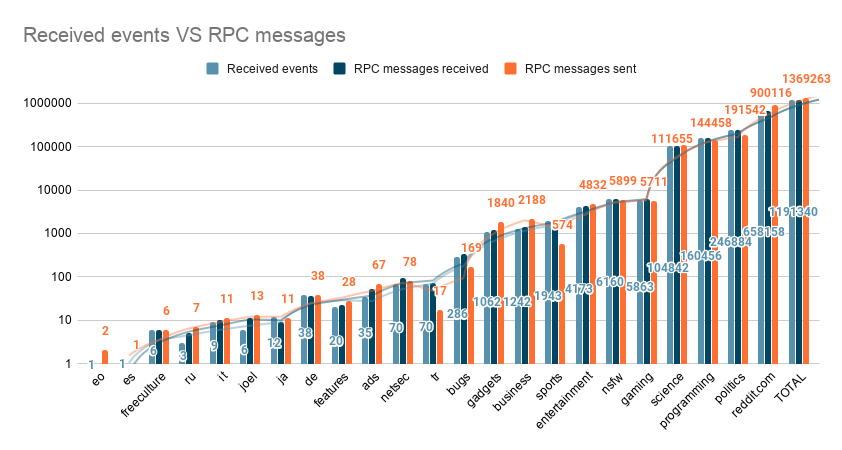
\includegraphics[width=0.8\textwidth]{img/graph-pulsarcast-latency-rpc.png}
  \caption{Pulsarcast without order guarantee and latency - Comparison of events received and \acrshort{rpc} injected in the system}
  \label{fig:graph-pulsarcast-latency-rpc}
\end{figure}

Just as it happened for all of our past experiments, Figure
\ref{fig:graph-pulsarcast-latency-rpc} shows us that the \acrshort{rpc}
messages injected in the system grow linearly with the number of events
received.

Table \ref{table:pulsarcast-latency} provides an overview of the Memory and
Network utilisation by node. Similar to the previous experiments, these grew
linearly throughout the test execution. As such, we are only presenting the
final values. We also provide an \acrshort{rpc} message analysis by node. Through this
table we can see how the duration of our test run impacted our resource
consumption, starting with the Memory usage and the Network bytes transmitted,
which were quite high in total compared to the same latency injected execution
with order guarantee. More than twice for our network transmission rate and
almost twice the memory usage.

Contrary to the other experiments we present the \acrshort{cpu} usage in a
table format in Table \ref{table:pulsarcast-latency-cpu} using ranges for both
time and \acrshort{cpu} number.  This is both for the sake of simplicity and
readability, given the \acrshort{cpu} usage followed a similar pattern as the
one we have seen in \ref{subsec:pulsarcast-with-order-guarantee-and-latency}.
Just as in that execution, we encounter a spiky behaviour, consequence of the
latency induced in the system. However, we experience an overall set of stable
values. With most of these inside a particular range throughout all the
execution. Similar to other executions, the spotted outliers can be explained,
as these were the nodes publishing messages at the time.

\begin{table}[!htb]
\caption{Pulsarcast without order guarantee and latency - Resource utilisation metrics per node}
\label{table:pulsarcast-latency}
  \begin{center}
   \begin{tabular}{|c| c c c c c|} 
    % \label{tab:pulsarcast-order}
   \hline
   / & P95 & P99 & Average & Standard Deviation & Total \\ [0.5ex] 
   \hline\hline
   Memory (\acrshort{gib}) & 0.41 & 0.43 & 0.36 & [NA] & 35.8 \\
   \hline
   Network (\acrshort{mib}) & 91.01 & 214.51 & 34.23 & [NA] & 3423 \\
   \hline
   \acrshort{rpc} Messages Received & 19624.35 & 19838.92 & 18773.3 & 2401.22 & [NA] \\
   \hline
   \acrshort{rpc} Messages Sent & 113367.75 & 412396.32 & 21756.75 & 64928.3 & [NA] \\ [1ex] 
   \hline
  \end{tabular}
  \end{center}
\end{table}

\begin{table}[!htb]
\caption{Pulsarcast without order guarantee and latency - \acrshort{cpu} utilisation across time, using ranges}
\label{table:pulsarcast-latency-cpu}
  \begin{center}
   \begin{tabular}{|c| c c c c|} 
    % \label{tab:pulsarcast-order}
   \hline
   Time Range & P95 & P99 & Average & Total \\ [0.5ex] 
   \hline\hline
   [0 - 1] & [0.01 - 0.04] & [0.1 - 0.02] & 0.01 & [0.6 - 1.25] \\
   \hline
   ]1 - 8[ & [0.01 - 0.04] & [0.03 - 0.06]  & 0.01 & [0.6 - 1.25] \\
   \hline
   8 & [0.01 - 0.05] & [0.03 - 0.06] & 0.01 & [0.6 - 1.25] \\
   \hline
   [8 - 13] & [0.01 - 0.04] & [0.03 - 0.06]  & 0.01 & [0.6 - 1.25] \\
   \hline
  \end{tabular}
  \end{center}
\end{table}

\subsection{Floodsub With Latency}\label{subsec:floodsub-with-latency}

Our last and final execution is a test run using Floodsub but with latency
induced through Toxiproxy. As previously all the nodes have an inbound latency
of 500 ms with 300 ms of jitter. The main goal for this test was for us to see
the behaviour of our baseline solution when under unfavourable network
conditions. It took a total of 60 minutes to finish. Similar to our test run in
Section \ref{subsec:floodsub}, the whole network was unable to cope with the
load of our execution. Ten minutes after our test started nodes became
unresponsive and either crashed or were repeatedly terminated by our Kubernetes
scheduler, eventually hitting a minimum of 14 nodes running. It took 40 minutes
for the network to fully recover and have 100 nodes running again.

\begin{figure}[!htb]
  \centering
  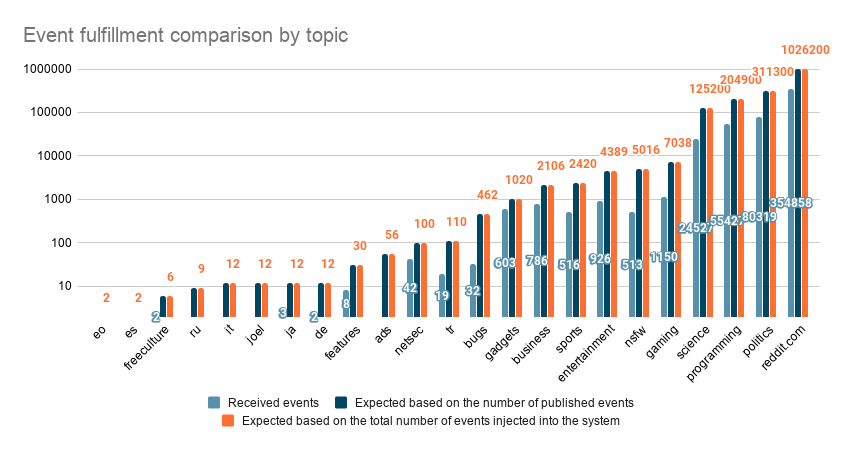
\includegraphics[width=0.8\textwidth]{img/graph-floodsub-latency-event-fulfillment-comparison.png}
  \caption{Floodsub with latency - Comparison of of events fulfilled by topic in a log scale}
  \label{fig:graph-floodsub-latency-event-fulfillment-comparison}
\end{figure}

\begin{figure}[!htb]
  \centering
  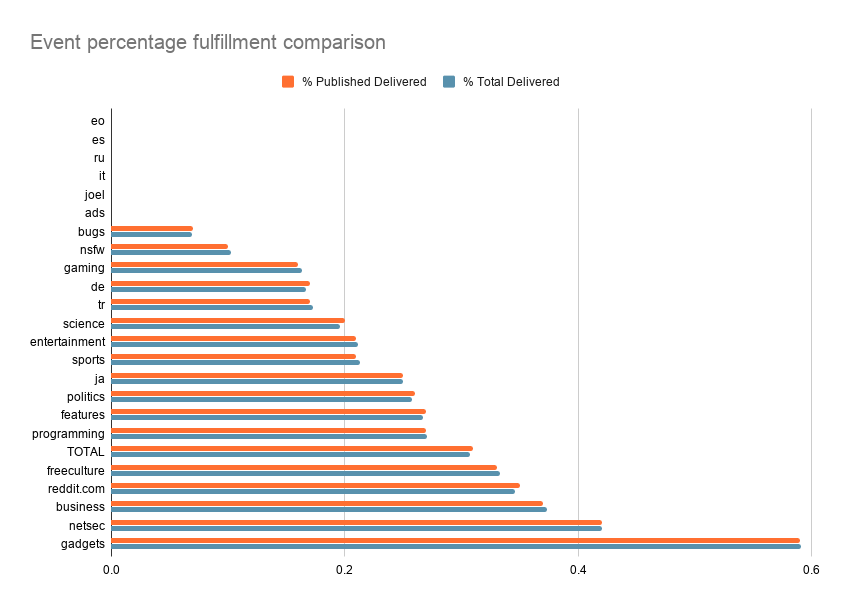
\includegraphics[width=0.8\textwidth]{img/graph-floodsub-latency-event-percentage-fulfillment-comparison.png}
  \caption{Floodsub with latency - Comparison of percentage of events fulfilled by topic}
  \label{fig:graph-floodsub-latency-event-percentage-fulfillment-comparison}
\end{figure}

Looking at \ref{fig:graph-floodsub-latency-event-fulfillment-comparison} and
\ref{fig:graph-floodsub-latency-event-percentage-fulfillment-comparison} we can
see that, of the total of events injected into the system, Floodsub fulfilled
31\% of its subscriptions as well as if we consider the events successfully
published as the base reference. Compared to the Floodsub experiment without
latency we see a drop of 10\% in subscription fulfilment.

\begin{table}[!htb]
\caption{Floodsub with latency - Resource utilisation metrics per node}
\label{table:floodsub-latency}
  \begin{center}
   \begin{tabular}{|c| c c c c|} 
    % \label{tab:pulsarcast-order}
   \hline
   / & P95 & P99 & Average & Total \\ [0.5ex] 
   \hline\hline
   Network (\acrshort{mib}) & 117.56 & 122.42 & 64.75 & 6474.79 \\
   \hline
  \end{tabular}
  \end{center}
\end{table}

\begin{figure}[!htb]
  \centering
  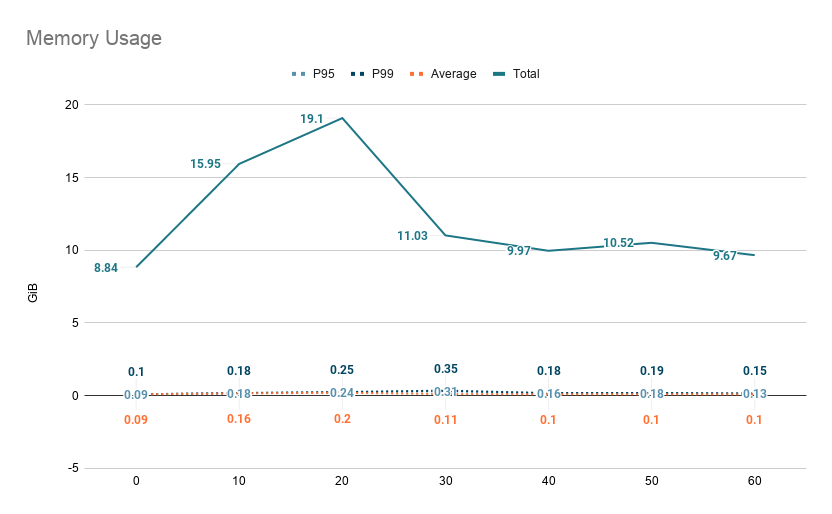
\includegraphics[width=0.8\textwidth]{img/graph-floodsub-latency-memory.png}
  \caption{Floodsub with latency - Memory usage across time}
  \label{fig:graph-floodsub-latency-memory}
\end{figure}

Table \ref{table:floodsub-latency} provides an overview of the Network
utilisation by node. As expected, it grew linearly during the test execution
and as such, we are only presenting the final values. Memory wise, it
fluctuated during the test (a consequence of the node failures) as such we are
presenting these values in the form of a graph in Figure
\ref{fig:graph-floodsub-latency-memory}.  The \acrshort{cpu} usage can be seen
in Figure \ref{fig:graph-floodsub-latency-cpu}. Starting by analysing the network
usage, we see a total value of 6475 \acrshort{mib} transmitted, averaging at 65
\acrshort{mib} by node.  Comparing with the latency-free execution, we again
see little to no difference at all. As expected, looking at memory and
\acrshort{cpu} usages, we see that the node crashes impacted these. Compared to
the latency-free execution, we do not see much changes other than a slight drop
in \acrshort{cpu} usage overall, probably a cause of the increased network
latency, which increased the \acrshort{cpu} idle time.

\begin{figure}[!htb]
  \centering
  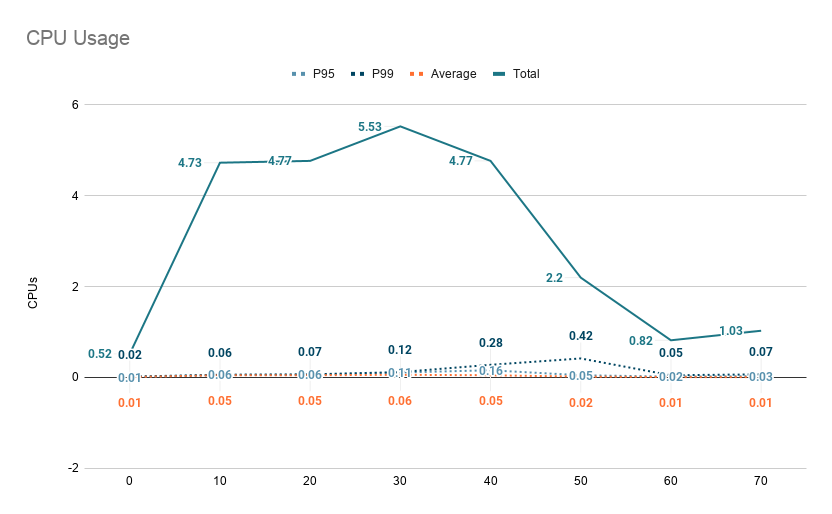
\includegraphics[width=0.8\textwidth]{img/graph-floodsub-cpu.png}
  \caption{Floodsub with latency - \acrshort{cpu} usage across time}
  \label{fig:graph-floodsub-latency-cpu}
\end{figure}

\subsection{Comparison and Discussion}\label{subsec:comparison}

In order to make our comparison easier, we have put into a tabular format a
summary of our test results for our multiple test runs in Table
\ref{table:evaluation-comparison}. We list:

\begin{itemize}
  \item Our coverage based on the total number of events we injected in the
    system
  \item Our coverage based on the total number of events effectively published
  \item Percentage of events effectively published
  \item Maximum total memory consumption in all of the system
  \item Network bytes transmitted in all of the system
  \item Maximum \acrshort{cpu} usage in all of the system
\end{itemize}

One aspect that we would like to highlight is the fact that we are not only
compressing months of data into a largely shorter timepsan, we are also
simulating interactions made by thousands of users into a much smaller set of
nodes (one hundred). All of this of course in an environment based on
virtualisation techniques and with a limited set of resources. This experiment
is essentially pushing the boundaries of what both systems would handle on a
real world scenario. It is also important to note that the percentage of events
actually published is not at all a useful metric for Floodsub, given no
acknowledgement whatsoever is made by the network when publishing an event,
making it irrelevant.

Looking at Floodsub as our baseline of comparison it is safe to say that
Pulsarcast surpassed Floodsub in every aspect, providing a better
\acrshort{qos} with a smaller resource footprint.  The only exception being the
total subscription coverage for Pulsarcast with order guarantee compared to
Floodsub, but then again, we are aiming at a different \acrshort{qos} level so
it makes this comparison quite unfair.  Resource wise, Floodsub is far more
network-intensive than Pulsarcast (with six times more usage in some cases) and
generally requires more \acrshort{cpu} power, even when compared to our order
guarantee scenarios. As expected though, Pulsarcast consumes more memory (when
comparing the latency induced executions, twice as much), a consequence  of the
\acrshort{qos} we want to offer and not persisting state into disk for our
executions.

Finally, one crucial property of Pulsarcast that is important to remember is
that, for every event effectively published, we store it in the \acrshort{dht}.
So, it is possible for any application using Pulsarcast to resolve past or
missing events from the event tree. This is the cornerstone of Pulsarcast's
eventual delivery guarantees, hence why it is essential to look at the
percentage of events effectively published as well as the subscription coverage
for these same events. Taking those same numbers into consideration we can see
a considerably high coverage percentage, with the lowest being 62\% for the
order guarantee test with latency injected.

\begin{sidewaystable}
\caption{Comparison table between our test executions}
\label{table:evaluation-comparison}
  \begin{center}
   \begin{tabular}{|l| c c c c c c|} 
    % \label{tab:pulsarcast-order}
   \hline
   / & Sub. Coverage &  Sub. Coverage for Published & Effectively Published &
   Memory(\acrshort{gib})* & Transmitted(\acrshort{mib})* & \acrshort{cpu}(\acrshort{vcpu})* \\ [0.5ex] 
   \hline\hline
   Floodsub & 41\% & 41\% & \textbf{100\%} & 21.15 & 6552.4 & 5.53 \\
   Pulsarcast & \textbf{99.99\%} & \textbf{99.99\%} &  \textbf{100\%} & 31.92 & 2237.74 & \textbf{3.77} \\
   Pulsarcast Order G. & 37\% & 82\% & 46\% & \textbf{17.84} & \textbf{1050.4} & 4.35 \\
   \hline
   Floodsub w/ Lat. & 31\% & 31\% & \textbf{100\%} & \textbf{15.95} & 6474.79 & 4.74 \\
   Pulsarcast w/ Lat. & \textbf{52\%} & \textbf{86\%} & 60\% & 35.8 & 3423 & \textbf{1.26}\\
   Pulsarcast Order G. w/ Lat. & 32\% & 62\% & 53\% & 19.99 & \textbf{1595.6} & 4.33 \\
   \hline
  \end{tabular}
  \footnotesize{*max values for the total system (sum of all the resources per node)}
  \end{center}
\end{sidewaystable}
